% Chapter Template
\chapter{Literature Review}
\label{Literature Review} % Change X to a consecutive number; for referencing this chapter elsewhere, use \ref{ChapterX}

%----------------------------------------------------------------------------------------
%   BACKGROUND
%----------------------------------------------------------------------------------------

\section{Background}

My thesis aims to investigate a form of task automation which links the technologies of the Internet of Things (IoT) and unmanned micro aerial vehicles (MAVs). These topics span across many disciplines, ranging from telecommunications to aeronautical engineering. Therefore, it is important that previous and current research in these areas is sufficiently reviewed before undertaking my own research.

%-----------------------------------
%       AUTOMATION
%-----------------------------------
\subsection{Automation}

Currently, automation in the future workforce is in the eye of the public and at the forefront of much innovation, policy and research (Edmonds 2015). Amongst other factors, the relative cost and unreliability of human workers when compared to computers is driving companies to automate operations. Recent examples range from the transport and logistics of goods (CNET 2014) to the synthesis of written media content (Smith 2015). According to CEDA (2015), 39.6\% of the current jobs in Australia have a high probability of ‘computerisation’. Autor, Levy and Murnane (2003) argue that “computer capital substitutes for workers in performing cognitive and manual tasks that can be accomplished by following explicit rules”.

%-----------------------------------
%       TELEMETRY
%-----------------------------------

\subsection{Telemetry}
The word, ‘telemetry’ is made up the components ‘tele-’ meaning ‘far off, afar, at or to a distance’ and ‘-metry’ meaning ‘meter, measure, or measurement’. Therefore, it involves the measurement of a physical quantity from a location different to that of the source. This practice has been around for almost 100 years, with (Linder 1929) outlining the then current methods of “telemetering” and supervisory control of energy generation, transmission and distribution. In many other applications, being able to quantify parameters of a system remotely is crucial to the system functioning properly.

One such telemetry task that has already begun to be automated is meter reading. In 2013, an Australian company, Taggle, reports that they have deployed a low-power WAN consisting of more than 100,000 motes with customers across the country (Taggle 2016). Their primary product is an internet-connected water meter able to be retrofitted to existing water meters. This solution employs the GSM cellular network, used primarily for voice and data signals of mobile phones, to transfer data from sensors to the internet.

However, there may be sensors embedded in many other forms of infrastructure that don’t have access to the cellular mobile network due to their remote location.

%----------------------------------------------------------------------------------------
%   THE INTERNET OF THINGS
%----------------------------------------------------------------------------------------

\section{The Internet of Things}

Wireless sensor networks (WSNs) form the back-bone of the Internet of Things. According to the IEC (2016), “A wireless sensor network is a network formed by a large number of sensor nodes where each node is equipped with a sensor to detect physical phenomena such as light, heat, pressure, etc.”. WSNs are discussed in detail in Wireless Sensor Networks.
However, the IoT is much more than just the hardware. In 1999, Kevin Ashton was believed to have been the first to use the term Internet of Things (IoT). He explained that his intended meaning was about connecting physical things to the digital world, as is only natural for physical people (Ashton 2009). Rose (2014) describes the connected nature of these things as making them ‘enchanted’. By the idea of ‘enchanted objects’, he means the creation of ordinary things that have extra-ordinary capabilities. Some examples given include a mirror that can aid one’s fashion decision in a fitting room, an umbrella that knows the weather forecast, or a garbage bin that encourages its user to live sustainably.

\begin{figure}
    \centering
    \includegraphics{iot-elements.jpg}
    \caption{Elements of the Internet of Things (Al-Fuqaha et al. 2015)}
    \label{fig:iot-elements}
\end{figure}

It is important to understand where my research topic fits in the scheme of the Internet of Things. Even though a fully-integrated solution will not be developed in this project, an experimental prototype is planned to connect physical quantities to the most basic of a digital ecosystem using a single-board computer.

This research covers the first 3 elements of an IoT solution, aiming to identify, sense and communicate data to and from wireless sensor nodes.

%----------------------------------------------------------------------------------------
%   MICRO AERIAL VEHICLES
%----------------------------------------------------------------------------------------

\section{Micro Aerial Vehicles}

Micro aerial vehicles (MAVs), or drones as they are referred to in the media, have been used for many novel applications – ranging from disaster relief to taking remote-control self-portraits (Lily Robotics 2015). They come in many varieties which generally fall under two categories: rotary- and fixed-wing.

MAVs are a subset of unmanned aerial vehicles (UAVs) which are of a reduced size compared to full-size autonomous aeroplanes such as military drones. Due to their size, MAVs lend well to research applications in which space is of the essence. Given a variety of payloads and sensor suites, these versatile aerial platforms have enabled much innovative research.
For example, a research centre in Switzerland have created a swarm of ‘ultra-light’ MAVs that dynamically link to each other in a mesh network configuration (Jimenez-Pacheco et al. 2012).
The UAV Challenge 2016 competition held in outback Australia focused on the development of a UAV or MAV to retrieve a blood sample from a house-ridden patient located in a remote location (BBC 2016). In both of these examples we see MAVs transporting something, whether it’s data or a physical blood sample.

%----------------------------------------------------------------------------------------
%       ROTARY WING
%----------------------------------------------------------------------------------------

\subsection{Rotary Wing}

Recently there has been explosion of rotary-wing type platforms, multi-rotors, popping up on crowd-funding platforms such as Kickstarter, and Indiegogo with many a novel and not-so-novel applications. These platforms are traditionally used for short and fast flights where the ability to hover in-place and perform a vertical take-off and landing (VTOL) are essential.

The most common COTS multi-rotor configuration is the 4-bladed ‘quadcopter’. This relies on the independent control of 4 vertically mounted brushless DC motors at the vertices of a quadrangle. Having 4 motors allows for redundancy of 1 motor, with an emergency landing manoeuvre able to be performed in the event of that occurring. A flight controller is necessary to fly these devices manually due to the inherent unstable nature of the system, which complicates the system. Due to their demand for electrical power, quadcopters are almost always powered by energy dense lithium-polymer batteries, typically ranging from 12.6 to 16.8 volts (3S and 4S packs).

\begin{figure}
    \centering
    \includegraphics{3dr-iris.jpg}
    \caption{Image of the IRIS+ multi-rotor development platform (3DR 2016)}
    \label{fig:3dr-iris}
\end{figure}

These types of platforms only have a nominal flight time of 20 minutes, making them very power hungry. This is due to a trade-off between manoeuvrability and endurance. The ability to hover and to land is ideal for densely populated areas with many trees and buildings.

Another type of rotary wing platform includes the traditional helicopter configuration, with a single rotor to provide upwards lift (and thrust) and a tail rotor to control yaw movement. This setup is mechanically more complex than a multi-rotor due to the variable pitch blades and swashplate mechanism, but it has proven to be a robust system for many decades on passenger helicopter systems.

%----------------------------------------------------------------------------------------
%       FIXED WING
%----------------------------------------------------------------------------------------

\subsection{Fixed Wing}

Fixed-wing platforms are less nimble, but far more stable and have incredible endurance relative to their similarly-sized hovering counterparts (Wasnak 2001). This is due to the aerofoil design of a wing, providing the lift force proportional to the airspeed. Due to this requirement of sufficient airspeed, fixed-wing platform aren’t able to hover in place, eliminating them from certain applications such as precise surveillance in enclosed areas. As with multi-rotors, there is a trade-off between manoeuvrability and endurance. The larger the wing, the more lift is generated as the plane flies, but that also leads to extra weight. Therefore, a low wing loading is required to maximise performance for long flights.

These platforms rely on a stable design, requiring minimal correction due to disturbances (such as gusts of wind) to increase flight efficiency. The stable design of a ‘flying wing’, for example, means that it, within reason, can level any roll disturbance with enough dihedral in the wing.
The number of control channels can be varied on a fixed-wing platform. A 4 channel platform means that the throttle (thrust), aileron (roll), elevator (pitch), and rudder (yaw) controls are in use. This provides the most control for a typical fixed-wing platform, not including the controls for flaps, retractable landing gear, or other miscellaneous functions. However, to simplify the amount of control inputs, a 3 channel system can be used, omitting yaw control. These systems are common in beginner model aircraft as they require less control inputs from the operator, and they also tend to be more stable with larger wings.

In the case of a flying wing, discrete control surfaces for the ailerons and elevator aren’t available and therefore must be ‘mixed’ into 2 control surfaces known as ‘elevons’. This system is still considered to be 3 channel, due to no vertical stabiliser being present for yaw control.

The power systems of fixed-wing drones can either be electric motors or miniaturised internal combustion (glow) engines. Modern MAV systems tend to be electrically powered. This may be due, in part, to researchers in control engineering being more familiar with electrical setups and not willing to learn the intricacies of internal combustion options. In addition to this, electrically powered MAVs allow clean, oil-free operation and can provide a more predictable performance across a range of weather conditions. Glow engines require fine manual tuning to optimise the fuel-to-air mixture which can become tedious and lead to unreliable flight times.

Aeromodellers have demonstrated that relatively cheap, fixed-wing MAVs can comfortably execute long-range flights of up to 4 kilometres, using specialised radio equipment for remote control and first-person video transmission.

\begin{figure}
    \centering
    \includegraphics{zeta-fx61.jpg}
    \caption{Zeta Science FX-61 Phantom fixed-wing platform}
    \label{fig:zeta-fx61}
\end{figure}

The commercially available platform for intermediate aeromodellers, Zeta Science FX-61 Phantom, exhibits the features of a long-endurance setup with a brushless DC motor power pod. This airframe is known to achieve flight times of up to an hour, when flown in a docile manner.

It is clear to use a fixed-wing MAV for long-range applications of acquiring and distributing data to wireless sensor nodes – with a flight path arranged to dwell around a mote for enough time to transfer data.

%----------------------------------------------------------------------------------------
%   WIRELESS COMMUNCATION
%----------------------------------------------------------------------------------------

\section{Wireless Communication}

Wireless communication was pioneered by Guglielmo Marconi, in which ‘telegraphic signals’ were transmitted via radio waves and received over a distance of an astonishing 29 kilometres, between Alum Bay, Isle of Wight and a steam-powered ship at sea. In his paper entitled Wireless Telegraphy, Marconi also describes the use cases of this new technology which included the regular updates from the Prince of Wales’ physician, aboard the Royal yacht, being received by a station located in Osborne House, at a transfer rate of about 15 words per minute (Marconi 1899).

\begin{figure}
    \centering
    \includegraphics{marconi-radio-tx.jpg}
    \caption{Early analogue radio transmitter (top) and receiver (bottom) apparatus (Marconi 1899)}
    \label{fig:marconi-radio-tx}
\end{figure}

This technology from the 1890’s required 40-metre-tall vertical wire installations for transmit and receive antennae, with bulky, high-powered apparatus located at the base of the structure, as shown Figure 4.

Unlike the fixed oscillation frequency used by Marconi, current radio technologies employ various bands of the electromagnetic spectrum to transmit analogue and digital signals across both long and short distances. Modern wireless communication technologies are largely designed for the transmission of digital messages, or packets, over the air between computing or storage devices. For higher transmission rate (bitrate) higher-frequency bands are utilised, such as the industrial, scientific, and medical (ISM) radio band.

The ISM band is used for “the operation of equipment or appliances designed to generate and use locally radio frequency energy for industrial, scientific, medical, domestic or similar purposes, excluding applications in the field of telecommunications” (ITU 2009). It includes the popular 2.4 GHz and 5.8 GHz frequencies used by many modern wireless communication protocols.

The following sections outline a few of the current wireless connectivity options, and address their relevance and fitness for use in the application of my research project.


%----------------------------------------------------------------------------------------
%   WIRELESS SENSOR NETWORKS
%----------------------------------------------------------------------------------------

\section{Wireless Sensor Networks}

This section outlines the different types of wireless sensor network topologies and challenges facing WSNs. The information contained in this section is adapted from Chapter 4: Sensor Network Topologies and Design Considerations of the book Sensor Technologies: Healthcare, Wellness and Environmental Applications (McGrath 2013).

%----------------------------------------------------------------------------------------
%       NETWORK TOPOLOGIES
%----------------------------------------------------------------------------------------

\subsection{Network Topologies}

A topology can be defined as the way in which constituent parts are interrelated or arranged. For WSNs, a network topology denotes the way in which motes are connected. Many different topologies have been developed for wireless sensor networks, with many resembling those of their previously wired counterparts. Each have their respective strengths and weaknesses. The following subsections briefly explain the 3 most relevant network topologies to the research topic. Hybrid topologies may be derived from the following, to leverage particular features of each for a given application.

%----------------------------------------------------------------------------------------
%       STAR
%----------------------------------------------------------------------------------------

\subsubsection{Star}

The star topology is named after the shape it creates when drawn as a 2-dimensional diagram. This approach relies solely on an intelligent central node sharing point-to-point connections with all other nodes. When implemented, this node is often considered the master and all others are treated as slaves. With many slave nodes, the master node may begin to create a bottleneck for the network and bandwidth may be limited from the slaves.

The master node is also a single point of failure, which may cause an issue for a critical system. Hence, redundancies must be engineered into the solution if a star topology is required.

\begin{figure}[h]
\centering
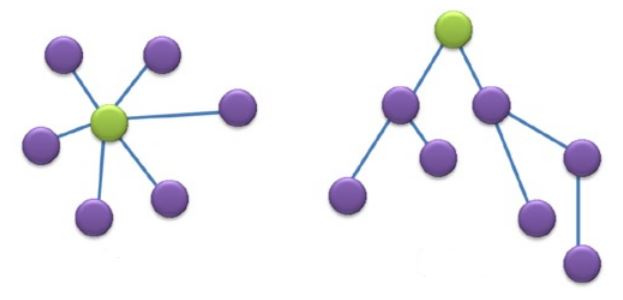
\includegraphics{Figures/star-tree-topology.JPG}
\decoRule
\caption[Star and tree network topologies]{Diagrams of star (left) and tree (right) topologies (McGrath 2013)}
\label{fig:StarTreeTopology}
\end{figure}

Bluetooth and Wi-Fi (IEEE 802.11) are household examples of technologies which utilise a star topology, with a smartphone or a wireless router playing the role of the central node and gateway.

%----------------------------------------------------------------------------------------
%       TREE
%----------------------------------------------------------------------------------------

\subsubsection{Tree}


The tree topology is also named after its geometric pattern resembling that of an upside-down tree. This is a hierarchical topology that includes a root node which acts as the gateway. Unlike the star topology, the nodes must be able to perform data aggregation and multi-hopping if it possesses a parent and child node. This requires the nodes to be more intelligent which increases processing power and power consumption.

Due to its ordered structure, it is easy to systematically debug and find faults when they occur. However, this introduces multiple points of failure other than the root node. If a node malfunctions, then all subsequent nodes will be rendered useless, despite functioning as normal. Therefore, the tree topology lacks the ability to re-configure and self-heal without the use of redundant nodes.

%----------------------------------------------------------------------------------------
%       MESH
%----------------------------------------------------------------------------------------

\subsubsection{Mesh}

The partially-connected mesh topology, when implemented intelligently, is arguably the most advanced of the WSN topologies due to it being dynamic in nature. Unlike the tree, all sensor nodes in this topology require all of the capabilities to multi-hop as outlined for the previous topologies, i.e. to pass data through a sensor node maintaining its source and directing to its destination.

Mesh networks are described as being self-healing, as data can be dynamically re-routed in the event of a node failure. This makes them desirable for many applications, including large-scale self-configurable networks which cover large areas and require minimal maintenance overhead.

\begin{figure}[h]
\centering
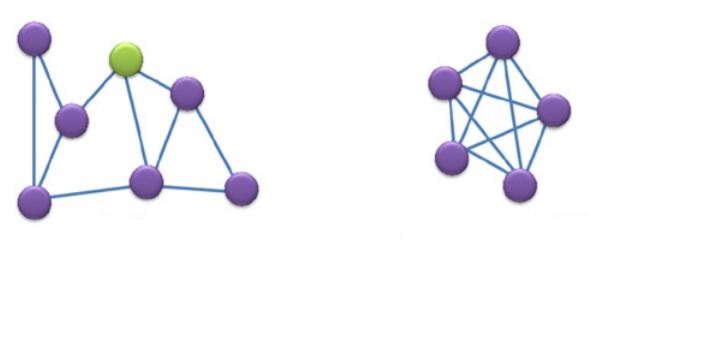
\includegraphics{Figures/mesh-fully-connected-mesh-topology.JPG}
\decoRule
\caption[Mesh and fully-connected mesh network topologies]{Diagrams of mesh (left) and fully-connected mesh (right) topologies (McGrath 2013)}
\label{fig:StarTreeTopology}
\end{figure}

Fully-connected mesh networks also consist of interconnected sensor nodes. However, each node must connect directly to all others, increasing data overhead and limiting the physical spread of the network.

A benefit of such a topology is that all nodes don’t require the ability to multi-hop due to the complete direct connections.

%----------------------------------------------------------------------------------------
%       PERSONAL AREA NETWORKS
%----------------------------------------------------------------------------------------

\subsection{Personal Area Networks}

Personal area networks (PANs) are classified by their limited scope and size of operation. The idea of the ‘quantified self’ has grown in recent times, and continues to increase in popularity. PANs are a network category specifically meant to wholly exist on one’s person. An everyday example of a common PAN is the connection between a smartphone in the pocket, wireless headphones, and a wearable activity tracker or smartwatch.

\subsubsection{Bluetooth}

Bluetooth® is a set of specifications maintained and updated by the Bluetooth® Special Interest Group (SIG), comprising hundreds of contributors across multiple technology companies. This specification operates on the 2.4 GHz ISM band, and utilises the star topology to connect a master to multiple slave devices.

The release of Bluetooth® v4.0 included new Bluetooth Smart™ (Low Energy) branding which indicates a new, low-power, reduced data-rate method of connectivity (Bluetooth® Core Specification 4.2 Quick Reference Guide 2014). This technology has given way to ultra-portable devices, powered by single-use coin cell batteries to last up to 2 or more years. Examples of BLE devices include wearables, most smartwatches, and beacons.

Beacons are compact, battery-powered, microcontroller devices that are Bluetooth® LE enabled. They act as an advertiser broadcasting packets without the need for pairing to another device. These packets are able to be sniffed by way of a scanner, which in this case is usually a smartphone.

\begin{figure}
    \centering
    \includegraphics{placeholder-image.jpg}
    \caption{Exploded view of an Estimote™ Proximity Beacon device}
    \label{fig:estimote-beacon-explode}
\end{figure}

Technology companies Apple and Google have jumped on board with this new development and created their own specifications for the advertisement frame to be broadcast by beacons, with iBeacon™ and Eddystone™ respectively. Another specification, AltBeacon™, has been developed by Radius Networks as an open-source alternative to iBeacon.

\begin{table}
    \centering
    \begin{tabular}{cccc}
        \hline \\
        Name & Author & Licence type & Specification \\
        \hline \\
        Eddystone™ & Google & Open-source & https://github.com/google/eddystone\\
        \hline \\
        iBeacon™ & Apple & Proprietary & https://developer.apple.com/ibeacon/ \\
        \hline \\
        AltBeacon™ & Radius Networks & Open-source &    https://github.com/AltBeacon/spec \\
        \hline \\
    \end{tabular}
    \caption{Bluetooth® LE Proximity Beacon specifications}
    \label{tab:ble-proximity-beacons}
\end{table}

\begin{figure}
    \centering
    \includegraphics{placeholder-image.jpg}
    \caption{iBeacon advertisement frame structure (ARM 2015)}
    \label{fig:ibeacon-ad-frame}
\end{figure}

The most common application of beacons to date is in the retail industry, to enable customer interaction via location-based notifications via smartphones. By method of triangulation, mobile apps are able to determine indoor location with the received signal strength indication (RSSI) from 3 or more beacons. For example, as a customer walks towards a promotional sale item, the store’s app may notify them or offer an even better, ‘exclusive’ offer at that moment.

Beacons can be installed en masse as markers on such things as public infrastructure like bus stops or train station platforms to enable contextually relevant content creation and notification to the user such as live bus or train ETAs. Beacons don’t attempt to replace GPS technology but rather supplement them to create a better experience inside and out. For example, Nearby Notifications, a product of Google, utilises BLE to allow “developers to tie an app or website to a BLE beacon and create contextual notifications, even with no app installed” (Google 2016).

Due to their application agnosticism, beacons are a curious technology that enables connection-less communication from an advertiser to a scanner. This proximity capability may pose helpful in the location of wireless sensor nodes via a flying vehicle to subsequently established a higher, enhanced data-rate connection via Bluetooth® or other point-to-point wireless communication protocol.

\subsubsection{Zigbee}

ZigBee® (IEEE 802.15.4-based) is a set of wireless communication specifications maintained by the ZigBee Alliance, which comprises of members Atmel, NXP, Philips, Silicon Labs, and many more. The standard is most commonly used in home automation products, powering connected homes by controlling lighting systems, transferring sensor data and security system information, or connecting smart appliances. The two most common specifications in use are ZigBee® PRO and ZigBee® RF4CE. The latter outlines a point-to-point RF communication protocol via 2.4 GHz ISM band, used for simple remote control applications such as garage doors and televisions. ZigBee® PRO will be investigated in more detail due to its advanced mesh networking capability.

\begin{figure}
    \centering
    \includegraphics{placeholder-image.jpg}
    \caption{ZigBee® PRO network topology (Digi 2016)}
    \label{fig:zigbee-pro-topology}
\end{figure}

Data is transmitted via the 2.4 GHz ISM band worldwide, and 915 MHz ISM band in the Americas. The 2.4 GHz version utilises direct-sequence spread spectrum (DSSS) modulation technique to overcome interference on the frequency band, achieving claimed ranges up to 3.2 kilometres outdoors (Digi 2016).

Networks are capable of containing up to 64,000 nodes in the current ZigBee PRO specification.

The ZigBee® PRO leverages the benefits of the partially-connected mesh network topology with multi-hop capability. There are 3 types of devices in a network, those include a ZigBee:

\begin{itemize}
    \item Coordinator - root node of the network and may be gateway to other types of networks (e.g. internet).
    \item Router - a multi-hop capable device performing its own application whilst also passing data through to other nodes.
    \item  End device - only capable of communicating with parent node in a star topology.
\end{itemize}

The selling points of ZigBee® are increased reliability, interoperability, and low-power operation. Reliability is achieved by the self-healing nature of mesh networks, eliminating any single points of failure. Interoperability is claimed, but this is only when different vendors create hardware that adheres to the ZigBee® standard.

For example, if a collection of connected light bulbs from different brands were installed, they could work cooperatively, listening to packets sent via a centralised controller or gateway. Low-power operation is achieved by the low data rate (20-250 kbps), coupled with the ability to broadcast data via a microcontroller within a very short period of time, enabling battery-less energy harvesting transmitter designs.

\subsection{Wireless Local Area Networks}

Wireless Local Area Networks (WLANs) are a wireless extension of the LAN, which is the term typically used to describe a network of computers inside a single building, office or home.

\subsubsection{Wi-Fi}

The most prominent WLAN technology is, of course, Wi-Fi® (IEEE 802.11), developed in part by the CSIRO. The technology is a set of media access control (MAC) and physical layer (PHY) specifications maintained by the IEEE Computer Society. Due to Wi-Fi®, we’ve seen the elimination of many Ethernet cables in computing device networks, and an increase in convenience for the everyday computer user. The most recent release, 802.11ac, has advertised data rates of at least 150 and 300 Mbps for the most basic of wireless routers.

Wi-Fi® and ZigBee® are commonly used together in residential and commercial dwellings due the rise in home automation products using the IEEE 802.15.4 standard. However, there has been notable interference experienced between the two technologies, since they both occupy the 2.4 GHz ISM band (Singh, Sharma \& Tomar 2013). Therefore, when mixing multiple wireless communication technologies, interference must be taken into account and tested prior to deployment.

\subsection{Low-Power Wide Area Networks}

A low-power wide area network (LPWAN), is a city-sized network that utilises low-power radio technologies to transmit data from motes to base station gateways located in a similar arrangement to GSM cellular network towers. LPWAN relies heavily on the base station infrastructure being installed adequately across the region to be connected. The motes connect to the base station in a star topology, meaning that the base station must service requests and receive data from hundreds to thousands of motes without overflowing an input buffer.

\subsubsection{LoRaWAN}

LoRaWAN is a media access control (MAC) specification for LPWANs which is maintained by the LoRa Alliance. Like the PAN and WLAN technologies, it utilises the ISM band for radio transmission. However, in Australia the 915-928 MHz band is used as opposed to 2.4 GHz.

It can achieve bitrates of 0.3 kbps to 50 kbps, using only 42.6 mA @ 3 V from the mote transceiver chipsets (such as the Microchip RN2903) in low-power low-range mode.

\begin{figure}
    \centering
    \includegraphics{placeholder-image.jpg}
    \caption{LoRaWAN block diagram (LoRa Alliance 2016)}
    \label{fig:lorawan-block-diagram}
\end{figure}

\subsubsection{NB-IoT}

Category M2 (3GPP Release 13) LTE is a very new specification released in Q1 2016. It has been called the narrow-band IoT (NB-IoT) technology due to its creation for use in IoT applications.

This method of creating LPWANs piggy backs of existing GSM cellular network towers, supposedly only requiring simple hardware upgrades to make them compatible with the new, low data-rate (250 kbps downlink, 250 or 20 kbps uplink) specification. It is said to the solve uplink limitations faced by competitor proprietary technology, Sigfox.

However, NB-IoT chipsets are yet to become commercially available, and require telecommunications companies to roll out infrastructure before deployment. Leveraging the reliability and security of a licenced service is appealing for IoT use cases.